\chapter{Sólidos e volumes}\label{ch:g9:solids}

A geometria do espaço começa com uma pequena família de \omterm{def:g5:solids:def}{sólidos} ---
\omterm{def:g7:areas:prism}{prismas}, \omterm{def:g7:areas:prism}{cilindros}, \omterm{def:g8:solids:def}{pirâmides}, \omterm{def:g8:solids:def}{cones}, esferas --- e duas perguntas:
quanto eles comportam (\omterm{def:g6:measure:volume}{volume}) e o que se vê quando são fatiados
(seções)? O capítulo se fecha com um fato de grande importância
prática: mudar a escala de um \omterm{def:g5:solids:def}{sólido} por $k$ multiplica o \omterm{def:g6:measure:volume}{volume} dele
por $k^3$.

\section{Os sólidos clássicos e os volumes deles}

\begin{theorem}[Fórmulas de volume]\label{thm:g9:solids:volumes}
Escreva $B$ para a \omterm{def:g6:measure:area}{área} da base e $h$ para a altura (a distância entre
a base e a \omterm{def:g5:solids:def}{face} oposta ou o \omterm{def:g5:solids:def}{vértice} do topo).
\begin{center}
\renewcommand{\arraystretch}{1.5}
\begin{tabular}{l|l}
\omterm{def:g5:solids:def}{sólido} & \omterm{def:g6:measure:volume}{volume} \\
\hline
\omterm{def:g7:areas:prism}{prisma}, \omterm{def:g7:areas:prism}{cilindro} & $V = B \times h$ \\[5pt]
\omterm{def:g8:solids:def}{pirâmide}, \omterm{def:g8:solids:def}{cone} & $V = \dfrac13\, B \times h$ \\[5pt]
esfera de \omterm{def:g3:shapes:shapes}{raio} $r$ & $V = \dfrac43\,\pi r^3$ \\
\end{tabular}
\end{center}
Para um \omterm{def:g7:areas:prism}{cilindro} e um \omterm{def:g8:solids:def}{cone} de \omterm{def:g3:shapes:shapes}{raio} $r$, a \omterm{def:g6:measure:area}{área} da base é
$B = \pi r^2$; a \omterm{def:g6:measure:area}{área} da superfície da esfera é $4\pi r^2$.
\end{theorem}
\admitted

\begin{omfigure}
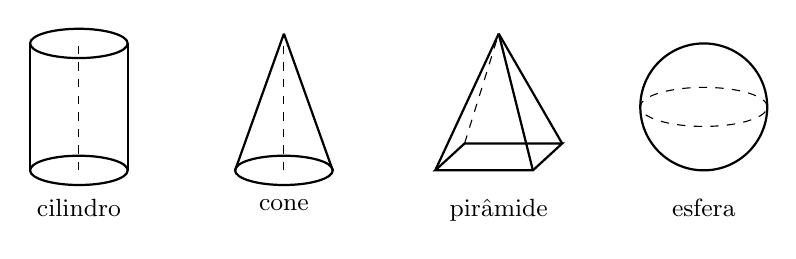
\begin{tikzpicture}[scale=0.62]
  % cilindro
  \draw[thick] (0,0) ellipse (1 and 0.3);
  \draw[thick] (-1,0) -- (-1,2.6);
  \draw[thick] (1,0) -- (1,2.6);
  \draw[thick] (0,2.6) ellipse (1 and 0.3);
  \draw[dashed] (0,0) -- (0,2.6);
  \node[below, font=\small] at (0,-0.4) {cilindro};
  % cone
  \begin{scope}[xshift=4.2cm]
  \draw[thick] (0,0) ellipse (1 and 0.3);
  \draw[thick] (-1,0) -- (0,2.8);
  \draw[thick] (1,0) -- (0,2.8);
  \draw[dashed] (0,0) -- (0,2.8);
  \node[below, font=\small] at (0,-0.4) {cone};
  \end{scope}
  % piramide
  \begin{scope}[xshift=8.4cm]
  \draw[thick] (-1.1,0) -- (0.9,0) -- (1.5,0.55) -- (-0.5,0.55) -- cycle;
  \draw[thick] (-1.1,0) -- (0.2,2.8);
  \draw[thick] (0.9,0) -- (0.2,2.8);
  \draw[thick] (1.5,0.55) -- (0.2,2.8);
  \draw[dashed] (-0.5,0.55) -- (0.2,2.8);
  \node[below, font=\small] at (0.2,-0.4) {pirâmide};
  \end{scope}
  % esfera
  \begin{scope}[xshift=12.8cm]
  \draw[thick] (0,1.3) circle (1.3);
  \draw[dashed] (0,1.3) ellipse (1.3 and 0.4);
  \node[below, font=\small] at (0,-0.4) {esfera};
  \end{scope}
\end{tikzpicture}

{\small Os \omterm{def:g5:solids:def}{sólidos} deste capítulo. Em cada um, o \omterm{def:g6:measure:volume}{volume} envolve uma
\omterm{def:g6:measure:area}{área} de base e uma altura --- menos na esfera, que só precisa do \omterm{def:g3:shapes:shapes}{raio}.}
\end{omfigure}

\begin{example}\label{ex:g9:solids:volumes}
Uma lata cilíndrica tem \omterm{def:g3:shapes:shapes}{raio} $4$ cm e altura $10$ cm:
\[
V = \pi r^2 h = \pi \times 16 \times 10 = 160\pi \approx 503
\text{ cm}^3 \approx 0.5 \text{ L}.
\]
Um \omterm{def:g8:solids:def}{cone} de mesma base e mesma altura comporta um terço disso:
$\frac{160\pi}{3} \approx 168$ cm$^3$. Uma esfera de \omterm{def:g3:shapes:shapes}{raio} $4$ cm:
$V = \frac43 \pi \times 64 = \frac{256\pi}{3} \approx 268$ cm$^3$.
\end{example}

\begin{example}[Uma pirâmide passo a passo]\label{ex:g9:solids:pyramid}
Uma \omterm{def:g8:solids:def}{pirâmide} tem base quadrada de lado $6$ m e altura $5$ m.
\begin{enumerate}
  \item \omterm{def:g6:measure:area}{Área} da base: $B = 6^2 = 36$ m$^2$.
  \item \omterm{def:g6:measure:volume}{Volume}: $V = \frac13 \times 36 \times 5 = 60$ m$^3$.
\end{enumerate}
Atenção às unidades: se o lado fosse dado em cm e a altura em m, um dos
dois teria de ser convertido antes.
\end{example}

\section{Seções por planos}

\begin{proposition}[Seções dos sólidos clássicos]\label{prop:g9:solids:sections}
Cortar um \omterm{def:g5:solids:def}{sólido} por um plano produz uma figura plana, a \emph{seção
transversal}\index{seção transversal} dele:
\begin{itemize}
  \item um \omterm{def:g7:areas:prism}{prisma} ou \omterm{def:g7:areas:prism}{cilindro} cortado \emph{paralelamente à base} dá
        uma cópia da base, em qualquer altura;
  \item uma \omterm{def:g8:solids:def}{pirâmide} ou um \omterm{def:g8:solids:def}{cone} cortado paralelamente à base dá uma
        \emph{redução} da base: à distância $d$ do \omterm{def:g5:solids:def}{vértice} do topo, o
        \omterm{def:g9:thales:scaling}{fator de escala} é $k = \frac{d}{h}$;
  \item uma esfera de \omterm{def:g3:shapes:shapes}{raio} $r$ cortada por um plano à distância
        $d < r$ do centro dá um círculo de \omterm{def:g3:shapes:shapes}{raio} $\sqrt{r^2 - d^2}$
        (pelo teorema de Pitágoras).
\end{itemize}
\end{proposition}
\admitted

\begin{omfigure}
\begin{tikzpicture}[scale=0.75]
  % cone com secao
  \draw[thick] (0,0) ellipse (1.5 and 0.45);
  \draw[thick] (-1.5,0) -- (0,4.0);
  \draw[thick] (1.5,0) -- (0,4.0);
  \draw[omThm, thick, fill=omThm!12] (0,2.4) ellipse (0.6 and 0.18);
  \draw[dashed] (0,0) -- (0,4.0);
  \node[right, font=\small] at (0.1,4.0) {vértice};
  \draw[Stealth-Stealth, thin] (2.1,0) -- (2.1,4.0);
  \node[right, font=\small] at (2.1,2.0) {$h$};
  \draw[Stealth-Stealth, thin, omThm] (0.9,2.4) -- (0.9,4.0);
  \node[right, font=\small, omThm] at (0.92,3.2) {$d$};
  % esfera com secao
  \begin{scope}[xshift=7.6cm]
  \draw[thick] (0,2) circle (1.8);
  \draw[omThm, thick, fill=omThm!12] (0,2.9) ellipse (1.56 and 0.4);
  \fill (0,2) circle (1.5pt) node[below, font=\small] {$O$};
  \draw[thin] (0,2) -- (0,2.9) node[midway, left, font=\small] {$d$};
  \draw[thin] (0,2.9) -- (1.56,2.9)
    node[midway, above, font=\small] {$\sqrt{r^2 - d^2}$};
  \draw[thin] (0,2) -- (-1.27,0.72)
    node[midway, below right=-3pt, font=\small] {$r$};
  \end{scope}
\end{tikzpicture}

{\small À esquerda: cortar um \omterm{def:g8:solids:def}{cone} paralelamente à base, à distância
$d$ do \omterm{def:g5:solids:def}{vértice}, dá um disco reduzido pelo fator $k = \frac dh$. À
direita: um plano à distância $d$ do centro de uma esfera a corta num
círculo de \omterm{def:g3:shapes:shapes}{raio} $\sqrt{r^2 - d^2}$.}
\end{omfigure}

\begin{example}\label{ex:g9:solids:section}
Um \omterm{def:g8:solids:def}{cone} tem \omterm{def:g3:shapes:shapes}{raio} da base $6$ e altura $9$. A seção por um plano
paralelo à base, à distância $3$ do \omterm{def:g5:solids:def}{vértice}, é um disco reduzido pelo
fator $k = \frac39 = \frac13$: o \omterm{def:g3:shapes:shapes}{raio} dele é $6 \times \frac13 = 2$.

Uma esfera de \omterm{def:g3:shapes:shapes}{raio} $5$ é cortada por um plano à distância $3$ do centro
dela: a seção é um círculo de \omterm{def:g3:shapes:shapes}{raio} $\sqrt{25 - 9} = 4$.
\end{example}

\section{Mudar a escala de sólidos}

\begin{theorem}[Efeito de uma mudança de escala sobre comprimentos, áreas e volumes]\label{thm:g9:solids:scaling}
Quando um \omterm{def:g5:solids:def}{sólido} é ampliado ou reduzido pelo fator de escala $k > 0$:
\begin{itemize}
  \item todos os comprimentos são multiplicados por $k$;
  \item todas as \omterm{def:g6:measure:area}{áreas} são multiplicadas por $k^2$;
  \item todos os \omterm{def:g6:measure:volume}{volumes} são multiplicados por $k^3$.
\end{itemize}
\end{theorem}
\admitted

\begin{example}\label{ex:g9:solids:scaling}
Um carrinho de coleção na escala $\frac{1}{18}$: os comprimentos são os
do carro de verdade multiplicados por $k = \frac{1}{18}$, a superfície
pintada é multiplicada por $k^2 = \frac{1}{324}$, e o \omterm{def:g6:measure:volume}{volume}, por
$k^3 = \frac{1}{5832}$.

Dobrar o \omterm{def:g3:shapes:shapes}{raio} de uma esfera ($k = 2$) multiplica o \omterm{def:g6:measure:volume}{volume} dela por
$2^3 = 8$: confira na fórmula,
$\frac43\pi (2r)^3 = \frac43 \pi \times 8r^3$.
\end{example}

\begin{example}[Tronco de cone]\label{ex:g9:solids:truncated}
Um \omterm{def:g8:solids:def}{cone} de altura $9$ e \omterm{def:g3:shapes:shapes}{raio} da base $6$ (\omterm{def:g6:measure:volume}{volume}
$\frac13 \pi \times 36 \times 9 = 108\pi$) é cortado à distância $3$ do
\omterm{def:g5:solids:def}{vértice}, e o \omterm{def:g8:solids:def}{cone} pequeno acima do corte é retirado. O \omterm{def:g8:solids:def}{cone} pequeno é a
redução pelo fator $k = \frac13$, então o \omterm{def:g6:measure:volume}{volume} dele é
$108\pi \times \left(\frac13\right)^3 = 4\pi$. O \omterm{def:g5:solids:def}{sólido} que resta (um
\emph{tronco de \omterm{def:g8:solids:def}{cone}}) tem \omterm{def:g6:measure:volume}{volume}
$108\pi - 4\pi = 104\pi \approx 327$.
\end{example}

\section{Exercícios}

\begin{exercise}[$\star$]\label{exo:g9:solids:1}
Calcule os \omterm{def:g6:measure:volume}{volumes}: uma caixa (\omterm{def:g7:areas:prism}{prisma} retangular) de dimensões
$4 \times 5 \times 12$; um \omterm{def:g7:areas:prism}{cilindro} de \omterm{def:g3:shapes:shapes}{raio} $3$ e altura $7$ (valor
exato com $\pi$ e depois arredondado à unidade).
\end{exercise}

\begin{exercise}[$\star$]\label{exo:g9:solids:2}
Calcule o \omterm{def:g6:measure:volume}{volume} de um \omterm{def:g8:solids:def}{cone} de \omterm{def:g3:shapes:shapes}{raio} $5$ e altura $12$ e o de uma
\omterm{def:g8:solids:def}{pirâmide} de base retangular $8 \times 3$ e altura $10$.
\end{exercise}

\begin{exercise}[$\star$]\label{exo:g9:solids:3}
Calcule o \omterm{def:g6:measure:volume}{volume} e a \omterm{def:g6:measure:area}{área} da superfície de uma esfera de \omterm{def:g3:shapes:shapes}{raio} $6$
(valores exatos com $\pi$).
\end{exercise}

\begin{exercise}[$\star$]\label{exo:g9:solids:4}
Uma esfera de \omterm{def:g3:shapes:shapes}{raio} $10$ é cortada por um plano à distância $8$ do
centro dela. Qual é o \omterm{def:g3:shapes:shapes}{raio} do círculo da seção?
\end{exercise}

\begin{exercise}[$\star\star$]\label{exo:g9:solids:5}
Um \omterm{def:g8:solids:def}{cone} tem \omterm{def:g3:shapes:shapes}{raio} da base $8$ e altura $12$. Um plano paralelo à base o
corta à distância $9$ do \omterm{def:g5:solids:def}{vértice}. Calcule o \omterm{def:g3:shapes:shapes}{raio} da seção e depois o
\omterm{def:g6:measure:volume}{volume} do \omterm{def:g8:solids:def}{cone} pequeno acima do corte.
\end{exercise}

\begin{exercise}[$\star\star$]\label{exo:g9:solids:6}
Um copo cilíndrico de \omterm{def:g3:shapes:shapes}{raio} interno $3$ cm contém água até a altura de
$10$ cm. Uma bola de \omterm{def:g3:shapes:shapes}{raio} $2$ cm é totalmente submersa nele. De quanto
sobe o nível da água? (O \omterm{def:g6:measure:volume}{volume} acrescentado se espalha pela \omterm{def:g6:measure:area}{área} da
base do copo; dê a subida exata e depois arredonde ao milímetro.)
\end{exercise}

\begin{exercise}[$\star\star$]\label{exo:g9:solids:7}
Uma receita enche uma fôrma esférica de \omterm{def:g3:shapes:shapes}{raio} $6$ cm. Você só tem uma
fôrma esférica de \omterm{def:g3:shapes:shapes}{raio} $3$ cm. Quantas fôrmas pequenas você consegue
encher? (Responda sem calcular explicitamente nenhum dos dois \omterm{def:g6:measure:volume}{volumes}.)
\end{exercise}

\begin{exercise}[$\star\star$]\label{exo:g9:solids:8}
A Grande \omterm{def:g8:solids:def}{Pirâmide} de Gizé tem base quadrada de lado aproximadamente
$230$ m e altura de cerca de $147$ m. Estime o \omterm{def:g6:measure:volume}{volume} dela e expresse-o
em milhões de metros cúbicos.
\end{exercise}

\begin{exercise}[$\star\star\star$]\label{exo:g9:solids:9}
Um funil em forma de \omterm{def:g8:solids:def}{cone}, de \omterm{def:g3:shapes:shapes}{raio} $6$ cm e altura $12$ cm, com o
\omterm{def:g5:solids:def}{vértice} para baixo, é enchido de água até a \omterm{def:g3:division:half}{metade} da \emph{altura}
(medida a partir do \omterm{def:g5:solids:def}{vértice}).
\begin{enumerate}
  \item Que \omterm{def:g9:fractions:fraction}{fração} do \omterm{def:g6:measure:volume}{volume} do funil fica cheia?
  \item Se, em vez disso, ele for enchido com \omterm{def:g3:division:half}{metade} do \emph{\omterm{def:g6:measure:volume}{volume}}
        de água, mostre que a altura $d$ da água satisfaz
        $\left(\frac{d}{12}\right)^3 = \frac12$ e dê $d$ ao milímetro
        ($\sqrt[3]{0.5} \approx 0.7937$).
\end{enumerate}
\end{exercise}

\section{Problema: a lápide de Arquimedes}

\begin{problem}[{Problema de fim de semana --- a esfera é dois terços
do cilindro dela (duas vezes), a pilha 1:2:3 e a lei do
quadrado--cubo, que proíbe gigantes}]
\label{pb:g9:solids:1}
Arquimedes demonstrou muitos teoremas, mas um o deixou tão orgulhoso
que ele pediu que a \emph{figura} correspondente fosse gravada no
túmulo dele: uma esfera encaixada no \omterm{def:g7:areas:prism}{cilindro} mais justo possível. Um
século depois, o escritor romano Cícero, procurando entre os arbustos
perto de Siracusa, reconheceu o túmulo ``pela esfera e pelo \omterm{def:g7:areas:prism}{cilindro}''.
Este problema recupera o que a gravura guarda --- um duplo milagre de
dois terços --- e depois segue \omterm{def:g6:measure:volume}{volumes} e superfícies
(\cref{thm:g9:solids:volumes}, \cref{thm:g9:solids:scaling}) até uma
lei que governa gigantes, formigas e planetas que esfriam.

\medskip
\noindent\textbf{Parte I --- A gravura decifrada.}
Uma esfera de \omterm{def:g3:shapes:shapes}{raio} $r$ fica exatamente dentro de um \omterm{def:g7:areas:prism}{cilindro}: mesmo
\omterm{def:g3:shapes:shapes}{raio}, altura $2r$.
\begin{enumerate}
  \item Calcule o \omterm{def:g6:measure:volume}{volume} do \omterm{def:g7:areas:prism}{cilindro} em função de $r$.
  \item Calcule a razão entre o \omterm{def:g6:measure:volume}{volume} da esfera e o do \omterm{def:g7:areas:prism}{cilindro}. Por
        que Arquimedes pode ter gostado do fato de a resposta não
        conter nem $\pi$ nem $r$?
  \item Agora as superfícies: compare a \omterm{def:g6:measure:area}{área} da superfície da esfera
        com a superfície \emph{total} do \omterm{def:g7:areas:prism}{cilindro} (a parte lateral mais
        as duas tampas). Que razão aparece --- de novo?
  \item O espaço vazio entre a esfera e o \omterm{def:g7:areas:prism}{cilindro} tem \omterm{def:g6:measure:volume}{volume}
        $2\pi r^3 - \frac43\pi r^3$. Mostre que essa sobra é exatamente
        igual ao \omterm{def:g6:measure:volume}{volume} de \emph{dois \omterm{def:g8:solids:def}{cones}} de \omterm{def:g3:shapes:shapes}{raio} $r$ e altura $r$.
  \item Uma bola de basquete de \omterm{def:g3:shapes:shapes}{raio} $12$ cm é vendida na caixa
        cilíndrica mais justa possível. Calcule os dois \omterm{def:g6:measure:volume}{volumes}
        (arredondando à centena de cm$^3$) e a porcentagem da caixa que
        fica vazia.
\end{enumerate}

\medskip
\noindent\textbf{Parte II --- Tigelas, fôrmas e luas.}
\begin{enumerate}[resume]
  \item Uma tigela hemisférica tem \omterm{def:g3:shapes:shapes}{raio} $10$ cm. Calcule a \omterm{def:g2:measure:units}{capacidade}
        dela, em cm$^3$ e em litros (ao decilitro).
  \item A pilha 1:2:3: um \omterm{def:g8:solids:def}{cone}, uma meia esfera e um \omterm{def:g7:areas:prism}{cilindro}, todos de
        \omterm{def:g3:shapes:shapes}{raio} $10$ cm e altura $10$ cm. Calcule os três \omterm{def:g6:measure:volume}{volumes} e
        verifique a lendária proporção $1 : 2 : 3$. (Arquimedes também
        teria apreciado esta.)
  \item Uma esfera de chocolate de \omterm{def:g3:shapes:shapes}{raio} $3$ cm é derretida numa fôrma
        cilíndrica de \omterm{def:g3:shapes:shapes}{raio} $3$ cm. Que altura o chocolate alcança?
        (\omterm{def:g9:fractions:fraction}{Fração} exata e depois ao milímetro.)
  \item O \omterm{def:g3:shapes:shapes}{raio} da Terra é de cerca de $6\,371$ km, e o da Lua, de cerca
        de $1\,737$ km. Calcule a razão entre os \omterm{def:g3:shapes:shapes}{raios} e depois --- com
        o \cref{thm:g9:solids:scaling} --- a razão entre os \omterm{def:g6:measure:volume}{volumes}:
        quantas Luas caberiam dentro de uma Terra oca, em \omterm{def:g6:measure:volume}{volume}?
  \item Do mesmo teorema: qual é a razão entre as \emph{\omterm{def:g6:measure:area}{áreas} de
        superfície} da Terra e da Lua? E, em geral, quando o \omterm{def:g3:shapes:shapes}{raio} de um
        balão dobra, o que acontece com o \omterm{def:g6:measure:volume}{volume} e com a superfície
        dele? Enuncie a \emph{lei do quadrado--cubo}: quando uma forma
        cresce, os \omterm{def:g6:measure:volume}{volumes} deixam as superfícies para trás.
\end{enumerate}

\medskip
\noindent\textbf{Parte III --- A lei do quadrado--cubo governa o
mundo.}
\begin{enumerate}[resume]
  \item O argumento de Galileu contra os gigantes: imagine um ser
        humano ampliado por um fator $10$, com as mesmas proporções.
        Por que fator o peso cresce (o peso acompanha o \omterm{def:g6:measure:volume}{volume})? Por
        que fator cresce a \omterm{prop:g9:solids:sections}{seção transversal} dos ossos (uma \omterm{def:g6:measure:area}{área})? Por
        que fator cresce, então, a \emph{pressão} sobre cada
        centímetro quadrado de osso --- e o que acontece com o gigante?
  \item A mesma lei ao contrário explica as proezas das formigas: a
        força acompanha a \omterm{prop:g9:solids:sections}{seção transversal} do músculo (uma \omterm{def:g6:measure:area}{área}), e o
        peso acompanha o \omterm{def:g6:measure:volume}{volume}. Para um animal $100$ vezes menor em
        todas as direções, por que fatores o peso e a força encolhem, e
        por que fator melhora a razão entre força e peso?
  \item O calor é produzido pelo \omterm{def:g6:measure:volume}{volume} do corpo e perdido pela
        superfície dele. Mostre que, para uma esfera, a razão entre
        superfície e \omterm{def:g6:measure:volume}{volume} é $\frac{3}{r}$, e calcule-a para $r = 1$ e
        $r = 2$. Quem esfria mais rápido, um camundongo ou um urso ---
        e por que os bebês precisam de touca no inverno?
  \item Duas laranjas esféricas, de \omterm{def:g3:shapes:shapes}{raios} $4$ cm e $5$ cm, são vendidas
        pelo mesmo preço. Calcule a razão entre os \omterm{def:g6:measure:volume}{volumes} delas: quanto
        mais laranja a grande entrega pelo mesmo dinheiro?
  \item Final: descreva com precisão o que a figura da lápide guarda
        --- os dois ``dois terços'' das questões 2 e 3 --- e responda a
        Cícero em uma frase: por que um matemático escolheria, entre
        todas as conquistas do gênio dele como engenheiro, uma esfera
        dentro de um \omterm{def:g7:areas:prism}{cilindro}?
\end{enumerate}
\end{problem}
